\section{Versuch 1 - Arbeitsbereich der Verfahren}
\label{Versuch_1}
Mit diesem Versuch soll der Zusammenhang zwischen Standort eines Probanden und Position des Blickziels (Targets) untersucht werden. Dazu wird eine Klassenzimmerumgebung simuliert, in der sowohl Standort als auch Blickziel relativ zur Kamera bekannt sind.\\
Als Messinstrument für die Versuche 1 und 2 wurde die Explorer 4K Actioncam verwendet, da sie eine hohe Auflösung bei ausreichend $FPS$ und eine $170^\circ$ Weitwinkel-Linse mit großer Schärfentiefe besitzt. Mit ihrer 2,7K Einstellung wird ein $2688 \times 1520$ Farbvideo mit $30FPS$ aufgezeichnet.\\
Allerdings ist die Bildqualität durch Pixelrauschen und Ähnliches deutlich schlechter als die Verkleinerung der Originalaufnahmen in den Datensätzen.
\subsection{Versuchsaufbau}
In einem Raum wurde die Kamera in $2,06m$ Höhe $31cm$ hinter den Targets so montiert, das der gesamte Raum im Fokus liegt. Als Targets wurden 9 Punkte auf einer Ebene markiert mit der Kamera im Zentrum. Die Anordnung der Targets ist in \autoref{img_aufbau_target_Test} dargestellt.\\
Als Position der Probanden wurde ein Rasterfeld mit $1m$ Kantenlänge im Raum eingezeichnet auf einer Fläche von $7 \times 11m$. Die Probanden stellten sich auf diesen Positionen auf um nacheinander alle Targets zu betrachten. 
\begin{figure}
	\centering
	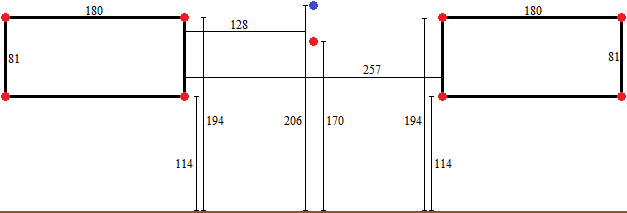
\includegraphics[width=0.7\linewidth]{img/Target}
	\caption{Aufbau der Targets im Vorversuch, alle Angaben gerundet in Zentimeter\\rote Punkte: Target, blauer Punkt: Kamera}
	\label{img_aufbau_target_Test}
\end{figure}
\subsection{Detektion mit MTCNN}
Um die Detektionswahrscheinlichkeit des MTCNN-Face Detektors zu testen wurden diese Videos analysiert.\\
Es zeigt sich, das auf allen Positionen die Probanden erfolgreich erkannt wurden und die Boxen das Gesicht recht gut beschreiben. Allerdings ist zu erkennen, das die Landmarks unzureichend genau sind. Sie sollten die Mundwinkel, Nasenspitze und beide Augen markieren, liegen aber schon bei recht großen Bildern weit daneben, siehe \autoref{img_bereich_MTCNN}
\begin{figure}
	\centering
	\begin{tabular}{|c|c|c|c|c|c|c|c|c|c|c|}
		\hline
		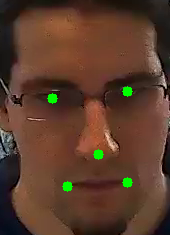
\includegraphics[width=1.1cm]{img_MTCNN/Img1-4_pupil1}&
		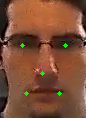
\includegraphics[width=1.1cm]{img_MTCNN/Img2-4_pupil1}&
		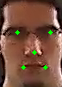
\includegraphics[width=1.1cm]{img_MTCNN/Img3-4_pupil1}&
		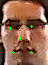
\includegraphics[width=1.1cm]{img_MTCNN/Img4-4_pupil1}&
		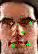
\includegraphics[width=1.1cm]{img_MTCNN/Img5-4_pupil1}&
		
\includegraphics[width=1.1cm]{img_MTCNN/Img6-4_pupil1}&
		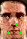
\includegraphics[width=1.1cm]{img_MTCNN/Img7-4_pupil1}&
		
\includegraphics[width=1.1cm]{img_MTCNN/Img8-4_pupil1}&
		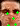
\includegraphics[width=1.1cm]{img_MTCNN/Img9-4_pupil1}&
		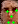
\includegraphics[width=1.1cm]{img_MTCNN/Img10-4_pupil1}&
		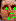
\includegraphics[width=1.1cm]{img_MTCNN/Img11-4_pupil1}\\
		\hline
		$1m$& $2m$& $3m$& $4m$& $5m$& $6m$& $7m$& $8m$& $9m$& $10m$& $11m$\\\hline
	\end{tabular}
	\caption{Dargestellt ist die Box und die 5 Landmarks von MTCNN-Face bei verschiedenen Distanzen des Probanden zur Actioncam}
	\label{img_bereich_MTCNN}
\end{figure}
\subsection{Auswertung der Aufnahme}
Für die Analyse wurden aus dem Video jene Frames ausgewählt in denen ein Target fokussiert wurde und analysiert.\\
Als erstes wurde die Einzelbildauswertung von OpenFace auf die Frames angewendet und jene Abbildungen der Kopfrotationen markiert, in denen erfolgreich ein Gesicht erkannt wurde. In \autoref{graph_Test_1_Normal} links ist der horizontale Wertebereich dargestellt in dem an der jeweiligen Position ein Gesicht erfolgreich erkannt wurde.\\
Im zweiten Teil wurden die selben Frames für die Messung verwendet, dieses mal allerdings wurde das gesamte Video analysiert. Der Winkelbereich in dem auf der horizontalen Achse an den entsprechenden Positionen ein Gesicht erkannt wurde, ist in \autoref{graph_Test_1_Normal} rechts dargestellt.\\
Um die grenzen Verbesserungen in einer Realen Umgebung auszutesten, wurde wie in \autoref{Implementierung_Ablauf} beschreiben vorgegangen und die relevanten Bildausschnitte linear vergrößert. Die Auswirkung auf den horizontalen Bereich ist in \autoref{graph_Test_1_Resize} dargestellt. Durch diese Verbesserung wird die Distanz auf der gearbeitet werden kann mehr als verdoppelt.
\begin{figure}
	\centering
	\begin{tabular}{ll}
	\begin{tabular}{|c|c|c|c|c|c|}
	\hline 
	$+6m$ & &&&&\\
	\hline 
	$+5m$ &
	
\includegraphics[width=0.5cm]{img_Bereich/V1_img_Winkel_X_-2000_5000.png} &
	
\includegraphics[width=0.5cm]{img_Bereich/V1_img_Winkel_X_-1000_5000.png} &
	
\includegraphics[width=0.5cm]{img_Bereich/V1_img_Winkel_X_0_5000.png} &
	
\includegraphics[width=0.5cm]{img_Bereich/V1_img_Winkel_X_1000_5000.png} &
	
\includegraphics[width=0.5cm]{img_Bereich/V1_img_Winkel_X_2000_5000.png} \\ 
	\hline 
	$+4m$ &
	
\includegraphics[width=0.5cm]{img_Bereich/V1_img_Winkel_X_-2000_4000.png} &
	
\includegraphics[width=0.5cm]{img_Bereich/V1_img_Winkel_X_-1000_4000.png} &
	
\includegraphics[width=0.5cm]{img_Bereich/V1_img_Winkel_X_0_4000.png} &
	
\includegraphics[width=0.5cm]{img_Bereich/V1_img_Winkel_X_1000_4000.png} &
	
\includegraphics[width=0.5cm]{img_Bereich/V1_img_Winkel_X_2000_4000.png} \\ 
	\hline 
	$+3m$ &
	
\includegraphics[width=0.5cm]{img_Bereich/V1_img_Winkel_X_-2000_3000.png} &
	
\includegraphics[width=0.5cm]{img_Bereich/V1_img_Winkel_X_-1000_3000.png} &
	
\includegraphics[width=0.5cm]{img_Bereich/V1_img_Winkel_X_0_3000.png} &
	
\includegraphics[width=0.5cm]{img_Bereich/V1_img_Winkel_X_1000_3000.png} &
	
\includegraphics[width=0.5cm]{img_Bereich/V1_img_Winkel_X_2000_3000.png} \\ 
	\hline 
	$+2m$ &&
	
\includegraphics[width=0.5cm]{img_Bereich/V1_img_Winkel_X_-1000_2000.png} &
	
\includegraphics[width=0.5cm]{img_Bereich/V1_img_Winkel_X_0_2000.png} &
	
\includegraphics[width=0.5cm]{img_Bereich/V1_img_Winkel_X_1000_2000.png} & \\ 
	\hline 
	$+1m$ & &
	
\includegraphics[width=0.5cm]{img_Bereich/V1_img_Winkel_X_-1000_1000.png} &
	
\includegraphics[width=0.5cm]{img_Bereich/V1_img_Winkel_X_0_1000.png} &
	
\includegraphics[width=0.5cm]{img_Bereich/V1_img_Winkel_X_1000_1000.png} & \\ 
	\hline 
	& $-2m$ & $-1m$ &0& $+1m$ & $+2m$ \\ 
	\hline 
\end{tabular}
	\begin{tabular}{|c|c|c|c|c|c|c|c|}
	\hline
	$+6$ &
	
\includegraphics[width=0.045\linewidth]{img_Bereich/V1_vid_Winkel_X_-3000_5000.png}&
	
\includegraphics[width=0.045\linewidth]{img_Bereich/V1_vid_Winkel_X_-2000_5000.png}&
	
\includegraphics[width=0.045\linewidth]{img_Bereich/V1_vid_Winkel_X_-1000_5000.png}&
	
\includegraphics[width=0.045\linewidth]{img_Bereich/V1_vid_Winkel_X_0_5000.png}&
	
\includegraphics[width=0.045\linewidth]{img_Bereich/V1_vid_Winkel_X_1000_5000.png}&
	
\includegraphics[width=0.045\linewidth]{img_Bereich/V1_vid_Winkel_X_2000_5000.png}&\\ 
	\hline 
	$+5$ &
	
\includegraphics[width=0.045\linewidth]{img_Bereich/V1_vid_Winkel_X_-3000_5000.png}&
	
\includegraphics[width=0.045\linewidth]{img_Bereich/V1_vid_Winkel_X_-2000_5000.png}&
	
\includegraphics[width=0.045\linewidth]{img_Bereich/V1_vid_Winkel_X_-1000_5000.png}&
	
\includegraphics[width=0.045\linewidth]{img_Bereich/V1_vid_Winkel_X_0_5000.png}&
	
\includegraphics[width=0.045\linewidth]{img_Bereich/V1_vid_Winkel_X_1000_5000.png}&
	
\includegraphics[width=0.045\linewidth]{img_Bereich/V1_vid_Winkel_X_2000_5000.png}&\\ 
	\hline 
	$+4$ &
	
\includegraphics[width=0.045\linewidth]{img_Bereich/V1_vid_Winkel_X_-3000_4000.png}&
	
\includegraphics[width=0.045\linewidth]{img_Bereich/V1_vid_Winkel_X_-2000_4000.png}&
	
\includegraphics[width=0.045\linewidth]{img_Bereich/V1_vid_Winkel_X_-1000_4000.png}&
	
\includegraphics[width=0.045\linewidth]{img_Bereich/V1_vid_Winkel_X_0_4000.png}&
	
\includegraphics[width=0.045\linewidth]{img_Bereich/V1_vid_Winkel_X_1000_4000.png}&
	\includegraphics[width=0.045\linewidth]{img_Bereich/V1_vid_Winkel_X_2000_4000.png}&
	\includegraphics[width=0.045\linewidth]{img_Bereich/V1_vid_Winkel_X_3000_4000.png}\\ 
	\hline 
	$+3$ &
	\includegraphics[width=0.045\linewidth]{img_Bereich/V1_vid_Winkel_X_-3000_3000.png}&
	\includegraphics[width=0.045\linewidth]{img_Bereich/V1_vid_Winkel_X_-2000_3000.png}&
	\includegraphics[width=0.045\linewidth]{img_Bereich/V1_vid_Winkel_X_-1000_3000.png}&
	\includegraphics[width=0.045\linewidth]{img_Bereich/V1_vid_Winkel_X_0_3000.png}&
	\includegraphics[width=0.045\linewidth]{img_Bereich/V1_vid_Winkel_X_1000_3000.png}&
	\includegraphics[width=0.045\linewidth]{img_Bereich/V1_vid_Winkel_X_2000_3000.png}&
	\includegraphics[width=0.045\linewidth]{img_Bereich/V1_vid_Winkel_X_3000_3000.png}\\ 
	\hline 
	$+2$ & &
	\includegraphics[width=0.045\linewidth]{img_Bereich/V1_vid_Winkel_X_-2000_2000.png}&
	\includegraphics[width=0.045\linewidth]{img_Bereich/V1_vid_Winkel_X_-1000_2000.png}&
	\includegraphics[width=0.045\linewidth]{img_Bereich/V1_vid_Winkel_X_0_2000.png}&
	\includegraphics[width=0.045\linewidth]{img_Bereich/V1_vid_Winkel_X_1000_2000.png}&
	\includegraphics[width=0.045\linewidth]{img_Bereich/V1_vid_Winkel_X_2000_2000.png}& \\ 
	\hline 
	$+1$ & & &
	\includegraphics[width=0.045\linewidth]{img_Bereich/V1_vid_Winkel_X_-1000_1000.png}&
	\includegraphics[width=0.045\linewidth]{img_Bereich/V1_vid_Winkel_X_0_1000.png}&
	\includegraphics[width=0.045\linewidth]{img_Bereich/V1_vid_Winkel_X_1000_1000.png}& &\\ 
	\hline 
	& $-3$& $-2$ & $-1$ &0& $+1$ & $+2$ & $+3$ \\ 
	\hline 
\end{tabular}
	\end{tabular}
	\caption{Dargestellt ist der horizontale Winkelbereich in denen ein Gesicht erkannt wurde.\\
	Links: Einzelbilder, Rechts: Video}
	\label{graph_Test_1_Normal}
\end{figure}
\subsection{Ergebnis}
Es zeigt sich, dass eine Auswertung von OpenFace auf einem Video deutlich zuverlässiger arbeitet als auf Einzelbildern, vor allem der größere Arbeitsbereich bezüglich der Rotation ist von Vorteil.\\
Durch die Verwendung des Weitwinkelobjektivs, kann die gesamte Breite eines Klassenzimmers erfasst werden und der Arbeitsbereich der Auswertung ist für eine erfolgreiche Detektion und Analyse breit genug um Schüler erfassen zu können, die selbst die vorderen Eckpunkte eines Klassenzimmers betrachten.\\
Bei der Distanz zur Kamera (Tiefe) besteht Handlungsbedarf, als Ziel wurde $8m$ angesetzt und das aktuelle Verfahren endet bei $5m$ in der einfachen Ausführung. Wird der Bildbereich allerdings verbessert, so verdoppelt sich die Distanz wischen Kamera und Person, wodurch eine Abdeckung des gesamten Klassenzimmers erreicht wird.\\
Der in \autoref{OpenFace_skal} theoretischen bestimmten Detektionsabstand von $14m$ konnte nicht erreicht werden, die erreichte Maximaldistanz liegt bei etwa $10m$, immer noch ausreichend für ein Klassenzimmer. Als Ursache kann das Pixelrauschen und die Überbeleuchtung durch das einfallende Licht der Fenster angenommen werden.\\
Auch MTCNN-Face ist als Detektor geeignet, er findet zuverlässige alle Gesichter im Frame, unabhängig ihrer Größe und Orientierung. Sogar jene die von OpenFace auch bei der Videoanalyse nicht verwendbar sind. Einzige Anmerkung ist die etwas ungenaue Box, dies kann aber mit einer einfachen Verschiebung der Boxränder korrigiert werden.\\
Eine signifikante Aussage bezüglich des vertikalen Winkel kann aus diesem Aufbau nicht getroffen werden, da die Neigungswinkel zwar differenziert werden können, sie allerdings zu ähnlich sind bei stehenden Personen (beides mal fast horizontal). Von Interesse ist ob ein Schüler auch erkannt werden kann, wenn dieser auf den Tisch vor sich schaut, was einen sehr großen Neigungswinkel bedeutet. Um dies aus zu testen wurde Versuch 2 durchgeführt.
\section{Versuch 2 - Arbeitsbereich der Verfahren}
Da ein aufmerksamer Schüler durchaus auch auf den Tisch blicken kann, z.B. beim Schreiben, soll getestet werden wie weit die Analyse in solchen Situationen funktioniert.
\subsection{Versuchsaufbau}
Für diesen Versuch wurde die Kamera auf $1,88m$ Höhe und $3m$ vor dem vordersten Standort der Probanden aufgestellt.\\
Als Standorte wurde eine Markierung mit einem Meter Abstand zueinander auf einer Gerade bei $3m$ und $9m$ verwendet.\\
Als Target diente die Kamera, ein Punkt $78cm$ unterhalb der Kamera und einer $40cm$ über dem Boden und $50cm$ vor der Kamera. Alle anderen Targets befinden sich $1m$ vor den Standorten.\\
Diesmal war das Versuchsgelände draußen an einem bedecken Tag, wodurch eine helle schattenlose Szene entsteht.
\subsection{Auswertung}
Es wurde die selbe Auswertung wie in Versuch 1 verwendet, einzelne Frames mit bekanntem Target. In \autoref{graph_Test_2_Normal} ist der vertikale Arbeitsbereich dargestellt, wiederum ist der Arbeitsbereich bei Verwendung der Video-Analyse etwas größer, wobei ein Winkel von $60^\circ$ nach unten erfasst werden kann.\\
Durch die Verbesserung der Eingabebilder kann auf einer Distanz von $9m$ gearbeitet werden, siehe \autoref{graph_Test_2_Resize}, mit dem Selben Arbeitsbereich.
\begin{figure}
	\centering
		\begin{tabular}{|c|c|c|c|c|c|c|c|c|}
	\hline 
	$+3m$ & &
	\includegraphics[width=0.5cm]{img_Bereich/V2_img_Winkel_Y_-2000_3000.png}&
	\includegraphics[width=0.5cm]{img_Bereich/V2_img_Winkel_Y_-1000_3000.png}&
	\includegraphics[width=0.5cm]{img_Bereich/V2_img_Winkel_Y_0_3000.png}&
	\includegraphics[width=0.5cm]{img_Bereich/V2_img_Winkel_Y_1000_3000.png}&
	\includegraphics[width=0.5cm]{img_Bereich/V2_img_Winkel_Y_2000_3000.png}&
	\includegraphics[width=0.5cm]{img_Bereich/V2_img_Winkel_Y_3000_3000.png}&\\ 
	\hline 
	& $-3m$ & $-2m$ & $-1m$ &Kamera& $+1m$ & $+2m$ & $+3m$ & $+4m$ \\ 
	\hline
	\hline 
	$+3m$ &
	\includegraphics[width=0.5cm]{img_Bereich/V2_vid_Winkel_Y_-3000_3000.png}&
	\includegraphics[width=0.5cm]{img_Bereich/V2_vid_Winkel_Y_-2000_3000.png}&
	\includegraphics[width=0.5cm]{img_Bereich/V2_vid_Winkel_Y_-1000_3000.png}&
	\includegraphics[width=0.5cm]{img_Bereich/V2_vid_Winkel_Y_0_3000.png}&
	\includegraphics[width=0.5cm]{img_Bereich/V2_vid_Winkel_Y_1000_3000.png}&
	\includegraphics[width=0.5cm]{img_Bereich/V2_vid_Winkel_Y_2000_3000.png}&
	\includegraphics[width=0.5cm]{img_Bereich/V2_vid_Winkel_Y_3000_3000.png}&
	\includegraphics[width=0.5cm]{img_Bereich/V2_vid_Winkel_Y_4000_3000.png}\\ 
	\hline 
	& $-3m$ & $-2m$ & $-1m$ &Kamera& $+1m$ & $+2m$ & $+3m$ & $+4m$ \\ 
	\hline 
\end{tabular}
	\caption{Dargestellt ist der horizontale Winkelbereich in denen ein Gesicht erkannt wurde.\\
		Oben: Einzelbilder, Unten: Video}
	\label{graph_Test_2_Normal}
\end{figure}
\begin{figure}
\centering
	\begin{tabular}{|c|c|c|c|c|c|c|c|c|}
	\hline 
	$+9m$ &
	\includegraphics[width=0.5cm]{img_Bereich/V2_img_res_Winkel_Y_-3000_9000.png}&
	\includegraphics[width=0.5cm]{img_Bereich/V2_img_res_Winkel_Y_-2000_9000.png}&
	\includegraphics[width=0.5cm]{img_Bereich/V2_img_res_Winkel_Y_-1000_9000.png}&
	\includegraphics[width=0.5cm]{img_Bereich/V2_img_res_Winkel_Y_0_9000.png}&
	\includegraphics[width=0.5cm]{img_Bereich/V2_img_res_Winkel_Y_1000_9000.png}&
	\includegraphics[width=0.5cm]{img_Bereich/V2_img_res_Winkel_Y_2000_9000.png}&
	\includegraphics[width=0.5cm]{img_Bereich/V2_img_res_Winkel_Y_3000_9000.png}&
	\includegraphics[width=0.5cm]{img_Bereich/V2_img_res_Winkel_Y_4000_9000.png}\\ 
	\hline 
	$+3m$ & &
	\includegraphics[width=0.5cm]{img_Bereich/V2_img_res_Winkel_Y_-2000_3000.png}&
	\includegraphics[width=0.5cm]{img_Bereich/V2_img_res_Winkel_Y_-1000_3000.png}&
	\includegraphics[width=0.5cm]{img_Bereich/V2_img_res_Winkel_Y_0_3000.png}&
	\includegraphics[width=0.5cm]{img_Bereich/V2_img_res_Winkel_Y_1000_3000.png}&
	\includegraphics[width=0.5cm]{img_Bereich/V2_img_res_Winkel_Y_2000_3000.png}&
	\includegraphics[width=0.5cm]{img_Bereich/V2_img_res_Winkel_Y_3000_3000.png}&
	\includegraphics[width=0.5cm]{img_Bereich/V2_img_res_Winkel_Y_4000_3000.png}\\ 
	\hline 
	& $-3m$ & $-2m$ & $-1m$ &Kamera& $+1m$ & $+2m$ & $+3m$ & $+4m$ \\ 
	\hline
	\hline 
	$+9m$ &
	\includegraphics[width=0.5cm]{img_Bereich/V2_vid_res_Winkel_Y_-3000_9000.png}&
	\includegraphics[width=0.5cm]{img_Bereich/V2_vid_res_Winkel_Y_-2000_9000.png}&
	\includegraphics[width=0.5cm]{img_Bereich/V2_vid_res_Winkel_Y_-1000_9000.png}&
	\includegraphics[width=0.5cm]{img_Bereich/V2_vid_res_Winkel_Y_0_9000.png}&
	\includegraphics[width=0.5cm]{img_Bereich/V2_vid_res_Winkel_Y_1000_9000.png}&
	\includegraphics[width=0.5cm]{img_Bereich/V2_vid_res_Winkel_Y_2000_9000.png}&
	\includegraphics[width=0.5cm]{img_Bereich/V2_vid_res_Winkel_Y_3000_9000.png}&
	\includegraphics[width=0.5cm]{img_Bereich/V2_vid_res_Winkel_Y_4000_9000.png}\\ 
	\hline 
	$+3m$ &
	\includegraphics[width=0.5cm]{img_Bereich/V2_vid_res_Winkel_Y_-3000_3000.png}&
	\includegraphics[width=0.5cm]{img_Bereich/V2_vid_res_Winkel_Y_-2000_3000.png}&
	\includegraphics[width=0.5cm]{img_Bereich/V2_vid_res_Winkel_Y_-1000_3000.png}&
	\includegraphics[width=0.5cm]{img_Bereich/V2_vid_res_Winkel_Y_0_3000.png}&
	\includegraphics[width=0.5cm]{img_Bereich/V2_vid_res_Winkel_Y_1000_3000.png}&
	\includegraphics[width=0.5cm]{img_Bereich/V2_vid_res_Winkel_Y_2000_3000.png}&
	\includegraphics[width=0.5cm]{img_Bereich/V2_vid_res_Winkel_Y_3000_3000.png}&
	\includegraphics[width=0.5cm]{img_Bereich/V2_vid_res_Winkel_Y_4000_3000.png}\\ 
	\hline 
	& $-3m$ & $-2m$ & $-1m$ &Kamera& $+1m$ & $+2m$ & $+3m$ & $+4m$ \\ 
	\hline 
\end{tabular}{\tiny }
	\caption{Dargestellt ist der horizontale Winkelbereich in denen ein Gesicht erkannt bei aufbereitetem Eingabebild.\\
	Links: Einzelbilder, Rechts: Video}
\label{graph_Test_2_Resize}
\end{figure}
\subsection{Ergebnisse}
Es zeigt sich, das eine Videoanalyse auch bei starker Neigung nach unten möglich ist. Die Einzelbildauswertung liefert erneut etwas schlechtere Ergebnisse als die Videoauswertung.\\
Dabei funktioniert das Tracking nur, wenn die Versuchsperson zuerst in die Kamera geschaut hat, um es zu beginnen. Aus diesem Test lässt sich ableiten, das auch eine Analyse erfolgen kann wenn der Schüler sich auf den Tisch vor ihm konzentriert.\\
Auch die stärkere gleichmäßige Beleuchtung ist hilfreich, da sie Probleme durch Gegenlicht und Schatten reduziert.
\section{Versuch 3 - Berechnung auf der Augenpartie}
Um einen Eindruck von ElSe mit hochauflösenden Aufnahmen zu erhalten, wurde ein weiterer Versuch durchgeführt mit einer deutlich bessern Kamera. Dieser Versuch soll auch die Nutzbarkeit von Eye-Tracking in solch einem Szenario testen.
\subsection{Versuchsaufbau}
Als Messinstrument wurde die Sony ILCE-6000 verwendet. Diese liefert ein $6000\times 4000$ Pixel großes Farbbild bei einer Brennweite von  $16mm$. Als Standort der Probanden wurden die selben wie in Versuch 1  verwendet. Da es sich um eine Fotokamera handelt, wurde ein Datensatz von Einzelbildern erstellt. Dabei wurden nur Aufnahmen gemacht, bei denen die Probanden direkt in die Kamera schauten.
\subsection{Auswertung}
Von Interesse ist die Augenpartie und die Ergebnisse des OpenFace Eye-Detektor im Vergleich zu ElSe, Dabei wurde ElSe in der Basiskonfiguration eingesetzt, dies bedeutet das Luminance-Verfahren, siehe \autoref{gray_Luminance} als Graukonvertierer und einem Radius der Maske von 12 Pixel.
Für die Analyse wurde zuerst mit OpenFace das Gesicht soweit analysiert um die Augenpartie als Eingabebild zu bestimmen, siehe \autoref{graph_Auge_Verbesserung} und ein Beispiel in \autoref{img_Versuch_Auge} oben. Auf diesem Eingabebild wird nun der ElSe-Algorithmus angewendet um die Ellipse zu bestimmen, dargestellt in grün. Im Vergleich sind die zusätzlichen 28 Landmarks der Augen von OpenFace auch in \autoref{img_Versuch_Auge} Mitte oben. Als Ergebnis wurde aus den berechneten Ellipsen von ElSe die Landmarks der Pupille und Iris abgeleitet und im selben Farbschema dargestellt.\\
Die einzelnen Augenpaare stammen von der selben Person, die sich bei der angegebenen Distanz frontal vor der Kamera befand. Es ist zu erkennen, das selbst bei einer hohen Auflösung die Augenpartie sehr klein ausfällt und nur schwierig auszuwerten ist.\\
Die Augenpartie der Probanden an den verschiedenen Positionen ist in \autoref{Augenbereich_Versuch3} dargestellt.
\begin{figure}
	\centering
	\begin {tikzpicture}
	\node[draw,align=center] (in) at(0,0) {Eingabebild\\\includegraphics[width=0.18\linewidth]{img_Versuch_Auge/Auge_in}};
	\node[draw,align=center] (El) at(6,0)  {Ellipse\\\includegraphics[width=0.18\linewidth]{img_Versuch_Auge/Auge_EL}};
	\node[draw,align=center] (OF) at(6,-4) {Landmark\\\includegraphics[width=0.18\linewidth]{img_Versuch_Auge/Auge_OF}};
	\node[draw,align=center] (ER) at(12,0)  {Ergebnis\\\includegraphics[width=0.18\linewidth]{img_Versuch_Auge/Auge_ER}};
		
	\draw[->] (in)to node[above]{ElSe}(El);
	\draw[->] (in)to node[left]{OpenFace}(OF);
	
	\draw[->] (El)to node[above]{Iris \& Pupille}(ER);
	\draw[->] (OF)to node[right]{Augenlider}(ER);	
\end{tikzpicture}
	\caption{Dargestellt sind der Ablauf, um die Landmarks des Auges zu verbessern}
	\label{graph_Auge_Verbesserung}
\end{figure}
\begin{figure}
	\centering
	\begin{tabular}{|c|c|c|c|c|c|c|c|c|c|c|} 
		\hline 
		\includegraphics[width=0.07\linewidth]{img_Versuch_Auge/Auge_2}&
		\includegraphics[width=0.07\linewidth]{img_Versuch_Auge/Auge_3}&
		\includegraphics[width=0.07\linewidth]{img_Versuch_Auge/Auge_6}&
		\includegraphics[width=0.07\linewidth]{img_Versuch_Auge/Auge_7}&
		\includegraphics[width=0.07\linewidth]{img_Versuch_Auge/Auge_10}&
		\includegraphics[width=0.07\linewidth]{img_Versuch_Auge/Auge_11}&	
		\includegraphics[width=0.07\linewidth]{img_Versuch_Auge/Auge_14}&
		\includegraphics[width=0.07\linewidth]{img_Versuch_Auge/Auge_15}&
		\includegraphics[width=0.07\linewidth]{img_Versuch_Auge/Auge_17}&
		\includegraphics[width=0.07\linewidth]{img_Versuch_Auge/Auge_19}&
		\includegraphics[width=0.07\linewidth]{img_Versuch_Auge/Auge_22}\\
		\hline 
		$1m$&$2m$&$3m$&$4m$&$5m$&$6m$&$7m$&$8m$&$9m$&$10m$&$11m$\\ 
		\hline 
	\end{tabular}
	\caption{Ergebnisse von OpenFace und ElSe bei verschiedenen Distanz.\\ Von Oben nach Unten: Augenparie, Ergebnis OpenFace, Ergebnis ElSe, ElSe Ergebnis als Landmarks}
	\label{img_Versuch_Auge}
\end{figure}
\subsection{Ergebnis}
Es zeigt sich, dass trotz einer hohen Bildauflösung der Informationsgehalt auf größere Distanzen deutlich abnimmt, wenn mit einer einzigen Kamera der gesamte Bereich einer Klasse erfasst werden soll. Außerdem ist auch gut zu erkennen, dass eine ausreichende Beleuchtung gebraucht wird, da die Augenregion sehr dunkel ausfällt.